\documentclass[handout]{beamer}
\usepackage[utf8]{inputenc}
\usepackage[T1]{fontenc}
\usepackage[french]{babel}
\usepackage{color}
\usepackage{fancyhdr}
\usepackage{lmodern}
\usepackage{makeidx}
\usepackage{graphicx}
\usepackage{amsmath}
\usepackage{amssymb}
\usepackage{mathrsfs}
\usepackage[bottom]{footmisc}

\usepackage{float}
\usepackage{textcomp}
\usepackage{verbatim}
\usepackage{ulem}
\usepackage{xcolor}
\usepackage{subfig}
\usepackage{hyperref}
\usepackage{subscript}

\hypersetup{
	colorlinks,
	linkcolor=blue,
}

\usepackage{multicol}
\setlength{\columnsep}{0.5cm}

\usetheme{ki}
\usefonttheme{serif}
\setbeamercolor{block title}{bg=blue!30,fg=black}
\setbeamertemplate{blocks}[rounded][shadow=true]


\title{Formation \LaTeX \vspace{0.2cm} Avancée}
\author{KI '020}
\institute{\color{white}Ecole des Ponts Paristech}
\date{\today}


% Commandes pour le TP
\newcommand{\THC}{tétrahydrocannabinol}
\newcommand{\formule}[3]{\textbf{C}\textsubscript{#1}\textbf{H}\textsubscript{#2}\textbf{O}\textsubscript{#3}}
\newcommand{\Deltatext}[1]{$\Delta$\up{#1}}

\begin{document}

	\begin{frame}
		\titlepage
	\end{frame}

	\begin{frame}
		\frametitle{Sommaire}
		\setcounter{tocdepth}{1}
		\tableofcontents
	\end{frame}

\section{Rappels (?)}

	\begin{frame}
		\frametitle{Quelques Rappels ?}
		\begin{itemize}
			\item Bibliographie ?
		\end{itemize}
	\end{frame}

	\begin{frame}[fragile=singleslide]
		\frametitle{Bibliographie}

		\centering
		Fichier .bib :
		\begin{verbatim}
			@book{ArchitectureHydraulique,
title={Architecture Hydraulique,
Ou l'Art de Conduire, d'Élever Et de Ménager Les Eaux},
author={Bernard Forest de Bélidor},
year={1737},
publisher={Charles-Antoine Jombert}
}
		\end{verbatim}

	\end{frame}

	\begin{frame}[fragile=singleslide]
		\frametitle{Bibliographie}
		\centering
		Pour citer au milieu du texte :\\

		\begin{verbatim}
			Pour savoir quelle machine choisir, il est donc nécessaire
			de trouver un moyen de comparer deux machines (ou moteurs)
			entre elles : Navier veut une unité de mesure qui
			représenterait les "quantités de travail employées pour
			effectuer toute espèce de fabrication"
			\cite{ArchitectureHydraulique}.
		\end{verbatim}

	\end{frame}

	\begin{frame}[fragile=singleslide]
		\frametitle{Bibliographie}

		\centering
		Fichier .bib importé à la fin du document \LaTeX :
		\begin{verbatim}
			\bibliographystyle{plain}
			\bibliography{fichier.bib}
		\end{verbatim}

	\end{frame}

	\begin{frame}

		\centering

		
\includegraphics[scale=0.45]{Images/Rappels/biblio.png}

	\end{frame}

	\begin{frame}[fragile=singleslide]
		\frametitle{Sommaire}

		\centering
		Pour avoir un sommaire tout bien tout fait :\\
		\begin{verbatim}
			\tableofcontents
		\end{verbatim}

		Pour ne pas garder les sous-sous-sections :

		\begin{verbatim}
		\setcounter{tocdepth}{2}
		\end{verbatim}

		\begin{tabular}{|c|c|c|c|}
			\hline
			-1 & Partie & 3 & Sous-sous-section\\ \hline
			0 & Chapitre & 4 & Paragraphe \\ \hline
			1 & Section & 5 & Sous-paragraphe \\ \hline
			2 & Sous-section & & \\ \hline
		\end{tabular}

	\end{frame}

	\begin{frame}
		\frametitle{Quelques Rappels ?}
		\begin{itemize}
			\item Bibliographie ?
			\item Inclure des images (notamment des images côte à côte) ?
		\end{itemize}
	\end{frame}

	\begin{frame}[fragile=singleslide]
		\frametitle{Inclure des images}

		\centering
		\begin{verbatim}
			\begin{figure}[options de position]
				\caption{\label{etiquette} titre}
			\includegraphics[options sur l'image]{chemin}
		\end{figure}
		\end{verbatim}

		Liste d'options de position :
		\begin{itemize}
			\item \textit{h} à côté du texte précédent la source
			\item \textit{t} en haut d'une page
			\item \textit{b} en bas d'une page
			\item \textit{p} dans une page ne contenant que des \emph{flottants} (images, tableaux, etc.)
			\item Avec le package \textit{float}, on peut utiliser \textit{H}
		\end{itemize}

	\end{frame}

	\begin{frame}
		\frametitle{Inclure des images}

		\centering
		Mettre côte à côte : utiliser un environnement \textit{tabular}...
	\end{frame}

	\begin{frame}[fragile=singleslide]
		\frametitle{Inclure des images}

		\centering
		Mettre côte à côte : utiliser un environnement \textit{tabular}... ou de nouveaux packages !\\

		\begin{verbatim}
			\usepackage{subfig}
		\end{verbatim}

	\end{frame}

	\begin{frame}[fragile=singleslide]
		\frametitle{Inclure des images}

		\begin{verbatim}
			\begin{figure}[h]
  \begin{center}
	\subfloat[Coco \& Moi]{
	  \includegraphics[width=0.3\textwidth]{regiscoco1.jpg}
	  \label{sub:campagnesbda}
						 }
	\subfloat[Moi \& Coco]{
	  \includegraphics[width=0.3\textwidth]{regiscoco2.jpg}
	  \label{sub:wei}
						 }
	\caption{C'était le WEI}
	\label{fig:cocomoi}
  \end{center}
\end{figure}
		\end{verbatim}

	\end{frame}

	\begin{frame}
		\frametitle{Inclure des images}

		\begin{figure}[h]
\begin{center}
\subfloat[Coco \& Moi]{
  \includegraphics[width=0.3\textwidth]{Images/Rappels/regiscoco1.jpg}
  \label{sub:campagnesbda}
					 }
\subfloat[Moi \& Coco]{
  \includegraphics[width=0.3\textwidth]{Images/Rappels/regiscoco2.JPG}
  \label{sub:wei}
					 }
\caption{C'était le WEI}
\label{fig:cocomoi}
\end{center}
\end{figure}
	\end{frame}

	\begin{frame}
		\frametitle{Quelques Rappels ?}
		\begin{itemize}
			\item Bibliographie ?
			\item Inclure des images (notamment des images côte à côte) ?
			\item Gérer l'indentation et la géométrie globale ?
		\end{itemize}
	\end{frame}

	\begin{frame}[fragile=singleslide]
	\frametitle{Formatage des paragraphes}

	\begin{enumerate}
		\item Changer les marges  de la page\\
			\begin{verbatim}
			\usepackage[a4paper,total={6in,8in}]{geometry}
			\end{verbatim}
	\end{enumerate}
\end{frame}

\begin{frame}[fragile=singleslide]
	\frametitle{Formatage des paragraphes}

	\begin{enumerate}
		\item Changer les marges  de la page\\

			\begin{verbatim}
			\usepackage[a4paper,total={6in,8in}]{geometry}
			\end{verbatim}
		\item Indentation d'un paragraphe\\

			\begin{verbatim}
			\setlength{\parindent}{4em}
			% (utiliser \indent et \noindent !)
			\end{verbatim}
	\end{enumerate}
\end{frame}

\begin{frame}[fragile=singleslide]
	\frametitle{Formatage des paragraphes}

	\begin{enumerate}
		\item Changer les marges  de la page\\
			\begin{verbatim}
			\usepackage[a4paper,total={6in,8in}]{geometry}
			\end{verbatim}
		\item Indentation d'un paragraphe\\

			\begin{verbatim}
			\setlength{\parindent}{4em}
			% (utiliser \indent et \noindent !)
			\end{verbatim}
		\item Distance inter-paragraphe\\

			\begin{verbatim}
			\setlength{\parskip}{1em}
			\end{verbatim}
	\end{enumerate}
\end{frame}

\begin{frame}[fragile=singleslide]
	\frametitle{Formatage des paragraphes}

	\begin{enumerate}
		\item Changer les marges  de la page\\

			\begin{verbatim}
			\usepackage[a4paper,total={6in,8in}]{geometry}
			\end{verbatim}
		\item Indentation d'un paragraphe\\

			\begin{verbatim}
			\setlength{\parindent}{4em}
			% (utiliser \indent et \noindent !)
			\end{verbatim}
		\item Distance inter-paragraphe\\

			\begin{verbatim}
			\setlength{\parskip}{1em}
			\end{verbatim}
		\item Hauteur de ligne\\
			\begin{verbatim}
			\renewcommand{\baselinestretch}{2}
			\end{verbatim}
	\end{enumerate}
\end{frame}

\begin{frame}
	\frametitle{Quelques Rappels ?}
	\begin{itemize}
		\item Bibliographie ?
		\item Inclure des images (notamment des images côte à côte) ?
		\item Gérer l'indentation et la géométrie globale ?
		\item Manier des structures de tableaux ?
	\end{itemize}
\end{frame}

\begin{frame}[fragile=singleslide]
	\frametitle{Tableaux}
	\centering
	Environnement \textit{tabular} :
	\begin{verbatim}
		\begin{tabular}{|l|c|r|}
			\hline
			colonne 1 & colonne 2 & colonne 3 \\
			\hline
			1 & 2 & 3\\
			\hline
		\end{tabular}
	\end{verbatim}

	\begin{tabular}{|l|c|r|}
		\hline
		colonne 1 & colonne 2 & colonne 3 \\
		\hline
		1 & 2 & 3\\
		\hline
	\end{tabular}

\end{frame}

\begin{frame}[fragile=singleslide]
	\frametitle{Tableaux}
	\centering
	Utilisation de \textit{multicolumn} :
	\begin{verbatim}
\begin{tabular}{|l|c|r|}
   \hline
   colonne 1 & \multicolumn{2}{c|}{colonnes 2 et 3} \\
   \hline
   1 & 2 & 3 \\
   \hline
   4 & 5 & 6 \\
   \hline
\end{tabular}
	\end{verbatim}

	\begin{tabular}{|l|c|r|}
	   \hline
	   colonne 1 & \multicolumn{2}{c|}{colonnes 2 et 3} \\
	   \hline
	   1 & 2 & 3 \\
	   \hline
	   4 & 5 & 6 \\
	   \hline
	\end{tabular}

\end{frame}

	\begin{frame}
		\frametitle{Quelques Rappels ?}
		\begin{itemize}
			\item Bibliographie ?
			\item Inclure des images (notamment des images côte à côte) ?
			\item Gérer l'indentation et la géométrie globale ?
			\item Manier des structures de tableaux ?
			\item Environnement mathématique ?
		\end{itemize}
	\end{frame}

	\begin{frame}[fragile=singleslide]
		\frametitle{Mathématiques}

		\centering
		Environnement \textit{\$ \$}:
		\begin{verbatim}
			$\frac{a}{b} \leq \sqrt[n]{2}$
			$$ \iiint_{\mathbb{R}^3} f(x,y,z)dxdydz $$
		\end{verbatim}

		$\frac{a}{b} \leq \sqrt[n]{2}$
		$$ \iiint_{\mathbb{R}^3} f(x,y,z)dxdydz $$

	\end{frame}

	\begin{frame}[fragile=singleslide]
		\frametitle{Mathématiques}
		\centering
		Environnement \textit{align, equation} :
		\begin{verbatim}
			\begin{equation}
				\cos(z)^2+\sin(z)^2 \neq 0
			\end{equation}
		\end{verbatim}

		\begin{equation}
			\cos(z)^2+\sin(z)^2 \neq 0
		\end{equation}


	\end{frame}

	\begin{frame}[fragile=singleslide]
		\frametitle{Mathématiques}
		\centering
		\begin{verbatim}
			\begin{align}
				\mathbb{E}(Z)
				&= \frac{1}{n}\sum_{i=1}^n \mathbb{E}(1)
				&= \exp(0)
			\end{align}
		\end{verbatim}

		\begin{align}
			\mathbb{E}(Z)
			&= \frac{1}{n}\sum_{i=1}^n \mathbb{E}(1)\\
			&= \exp(0)
		\end{align}

	\end{frame}

	\begin{frame}
		\frametitle{Quelques Rappels ?}
		\begin{itemize}
			\item Bibliographie ?
			\item Inclure des images (notamment des images côte à côte) ?
			\item Gérer l'indentation et la géométrie globale ?
			\item Manier des structures de tableaux ?
			\item Environnement mathématique ?
			\item Les bonnes pratiques pour travailler en groupe ?
		\end{itemize}
	\end{frame}

	\begin{frame}
		\frametitle{Gestion de projet}
		\begin{itemize}
			\item Utiliser des dépôts : Google Drive, Overleaf, GitHub, Trello
		\end{itemize}
	\end{frame}

	\begin{frame}
		\frametitle{Gestion de projet}
		\begin{enumerate}
			\item Utiliser des dépôts : Google Drive, Overleaf, GitHub, Trello
			\item Être rigoureux dans le code : warnings, erreurs, etc...
		\end{enumerate}
	\end{frame}

	\begin{frame}
		\frametitle{Gestion de projet}
		\begin{enumerate}
			\item Utiliser des dépôts : Google Drive, Overleaf, GitHub, Trello
			\item Être rigoureux dans le code : warnings, erreurs, etc.
			\item Rendez votre code clair : structurez, indentez, faites respirer le code
		\end{enumerate}
	\end{frame}

	\begin{frame}
		\frametitle{Gestion de projet}
		\begin{enumerate}
			\item Utiliser des dépôts : Google Drive, Overleaf, GitHub, Trello
			\item Être rigoureux dans le code : warnings, erreurs, etc.
			\item Rendez votre code clair : structurez, indentez, faites respirer le code
			\item Utiliser au maximum des IDEs avec des \textit{linters} et qui ont des modules d'autocomplétion
		\end{enumerate}
	\end{frame}

	\begin{frame}
		\frametitle{Gestion de projet}
		\begin{enumerate}
			\item Utiliser des dépôts : Google Drive, Overleaf, GitHub, Trello
			\item Être rigoureux dans le code : warnings, erreurs, etc.
			\item Rendez votre code clair : structurez, indentez, faites respirer le code
			\item Utiliser au maximum des IDEs avec des \textit{linters} et qui ont des modules d'autocomplétion
			\item Utiliser les moteurs de recherche au maximum pour de l'aide
		\end{enumerate}
	\end{frame}

\section{Faire de \textit{magnifiques} slides}


\begin{frame}[fragile=singleslide]
	\frametitle{Le type \textit{beamer}}
	\centering Ces slides sont faites en \LaTeX \hspace{0.1cm}avec le type \textbf{beamer}\\

	\begin{verbatim}
		\documentclass[handout]{beamer}
		\usepackage[utf8]{inputenc}
		\usepackage[T1]{fontenc}
		\usepackage[french]{babel}

		\usetheme{Warsaw}
		\usefonttheme{serif}
	\end{verbatim}
\end{frame}

\begin{frame}[fragile=singleslide]
	\frametitle{Le type \textit{beamer}}
	\centering
	Pour créer une slide :

			\begin{verbatim}
			\begin{frame}
			\frametitle{Titre de la slide}
			Contenu de la slide
			\end{frame}
			\end{verbatim}

\end{frame}

\begin{frame}[fragile=singleslide]
	\frametitle{Le type \textit{beamer}}
	\centering
	Pour partitionner les slides :\\
	L'environnement \textit{multi colonne}, \textit{minipage}, etc.

			\begin{verbatim}
			\usepackage{multicol}
			\setlength{\columnsep}{1cm}
			\end{verbatim}

\end{frame}

\begin{frame}[fragile=singleslide]
	\frametitle{Le type \textit{beamer}}
	\centering

			\begin{verbatim}
				\begin{multicols}{2}
				[
				\section{First Section}
				Titre de la section
				]
				Texte
				\end{multicols}
			\end{verbatim}

\end{frame}

\begin{frame}
	\frametitle{Le type \textit{beamer}}

	\begin{multicols}{2}
	[
	Les élèves de l'ENPC sont des êtres très touchants. Ils adorent être doux.
	]
	Ceci est le commencement de mon existence. Il s'avère que je suis né le 12 avril 1997. Et vous ? J'aime bien le sport : faire du sport, regarder du sport. Les fléchettes c'est marrant non ? On en apprend vraiment tous les jours sur le corps humain. D'ailleurs, j'aime beaucoup les corps de manière générale. Ce sont des choses impresionnantes. Vive l'amour.\\

	\indent Et hop, je reviens à la ligne.
	\end{multicols}

\end{frame}

\begin{frame}
	\frametitle{Le type \textit{beamer}}
	\framesubtitle{Ce qu'il est possible de faire avec ces environnements...}
	\centering
	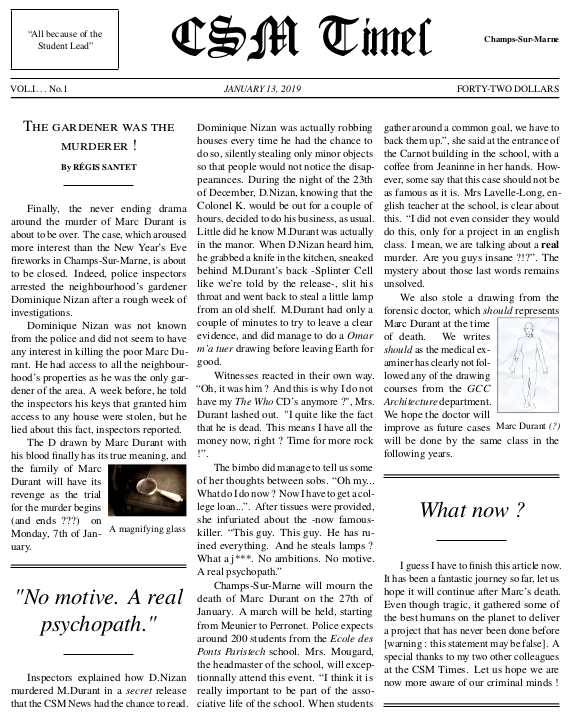
\includegraphics[scale=0.25]{Images/Beamer/column.png}
\end{frame}

\begin{frame}
	\frametitle{C'est l'heure du TP !}

	\begin{multicols}{3}
	[Preuve de l'existence de Dieu.]
	Alors que je me \textit{promenais} dans la rue, un vieux m'arrêta. ``Salutations, \textsc{humain} ! Voici ce que tu dois savoir :''\\
	\begin{equation*}
		H\Psi = E\Psi
	\end{equation*}
	Mon monde s'écroula. Non seulement je venais de comprendre mes erreurs, mais j'avais compris le but de toute chose. L'intrication quantique entre élèves des ponts n'était finalement pas seulement dûe au foyer...\\

	
\includegraphics[scale=0.1]{Images/Beamer/dieu.jpg}

	\end{multicols}

\end{frame}

\begin{frame}[fragile=singleslide]
	\frametitle{Solution}
	\begin{verbatim}
	\begin{frame}
	\frametitle{C'est l'heure du TP !}
	
	\begin{multicols}{3}
	[Preuve de l'existence de Dieu.]
	Alors que je me \textit{promenais} dans la rue, 
	un vieux m'arrêta. 
	``Salutations, \textsc{humain} ! Voici
	ce que tu dois savoir :''\\
	\begin{equation*}
	H\Psi = E\Psi
	\end{equation*}
	\end{verbatim}
	
\end{frame}

\begin{frame}[fragile=singleslide]
	\frametitle{Solution}
	\begin{verbatim}
	Mon monde s'écroula. Non seulement je
	venais de comprendre mes erreurs, mais
	j'avais compris le but de toute chose.
	L'intrication quantique entre élèves
	des ponts n'était finalement pas
	seulement dûe au foyer...\\
	
	
\includegraphics[scale=0.1]{Images/Beamer/dieu.jpg}
	\end{multicols}
	\end{frame}
	\end{verbatim}
\end{frame}

\begin{frame}[fragile=singleslide]
	\frametitle{Et les maths avec beamer ?}

	Souvent, on voit des boîtes qui entourent certains résultats importants :
	\begin{verbatim}
		\begin{block}{blocktitle}
			Chose importante méritant une attention particulière
		\end{block}
	\end{verbatim}

	Marche aussi avec \textit{\color{red}{alertblock}}, \textit{\color{green}{exampleblock}}.
\end{frame}

\begin{frame}
	\frametitle{Et les maths avec beamer ?}
	\vspace{-0.2cm}
	\begin{block}{Ratio de vraisemblance}
	    On introduit la statistique suivante :
	    $$
	    \begin{array}{ccl}
	    \Lambda(y_n|x_n) & = & 2\, \log\frac{\mbox{Maximum de vraisemblance du problème}}{\mbox{Maximum de vraisemblance sous } H_0} \\
	    & & \\
	    & = & 2\,\log \frac{\prod_{i=1}^n \hat{p}(1|x_i)^{y_i}(1-\hat{p}(1|x_i))^{1-y_i}}{\prod_{i=1}^n (\hat{p}^*)^{y_i}(1-\hat{p}^*)^{1-y_i}}
	    \end{array}
	    $$
	\end{block}

	\begin{block}{Lemme}
		Sous $H_0$, $\Lambda(y_n|x_n)$ converge en loi vers la distribution $\chi_2(1)$
	\end{block}

	\begin{block}{Corrolaire}
		On rejette $H_0$ si $\Lambda(y_n|x_n) \geq \chi_{1,1-\alpha}^2$ avec un niveau asymptotique $\alpha$.
	\end{block}

\end{frame}

\begin{frame}
	\frametitle{Petite sieste tactique}
	\Huge
	\centering

	PAUSE <3
\end{frame}

\section{Utiliser des templates}

\begin{frame}
	\frametitle{Bientôt dans votre scolarité}
	\centering
	Dans les différents départements (2A, DLC) et pour votre vie future :\\
	\begin{itemize}
		\item Faire des posters
		\item Faire votre CV
		\item Faire des articles, des thèses, etc.
	\end{itemize}
\end{frame}

\begin{frame}
	\frametitle{Utilisation des templates}

	\centering
	\Huge
	\fbox{\textsc{Templates}}
	\normalsize

	\hspace{2cm}

	\begin{itemize}
		\item \url{https://fr.overleaf.com/latex/templates}
		\item \url{https://fr.sharelatex.com/templates}
		\item \url{https://www.latextemplates.com/}
	\end{itemize}
\end{frame}

\section{Quelques trucs sympas}

\begin{frame}[fragile=singleslide]
	\frametitle{Inclure du \LaTeX}

	\centering

	\begin{verbatim}
		\usepackage{verbatim}

		\begin{verbatim}
			\begin{itemize}
				\item ...
			\end{itemize}
		%end{verbatim}

	\end{verbatim}

	Attention aux slides :\\
	\begin{verbatim}
		\begin{frame}[fragile=singleslide]
			stuff
		\end{frame}
	\end{verbatim}

\end{frame}

\begin{frame}[fragile=singleslide]
	\frametitle{Mettre un lien}

	\begin{enumerate}
		\item Faire des liens :\\
			\begin{verbatim}
			\url{https://en.wikibooks.org/wiki/LaTeX}
			\href{https://en.wikibooks.org}{Un lien}
			\end{verbatim}
	\end{enumerate}
\end{frame}

\begin{frame}[fragile=singleslide]
	\frametitle{Mettre un lien}

	\begin{enumerate}
		\item Faire des liens :\\
			\begin{verbatim}
			\url{https://en.wikibooks.org/wiki/LaTeX}
			\href{https://en.wikibooks.org}{Un lien}
			\end{verbatim}
		\item Rendre cliquable le sommaire :\\
			\begin{verbatim}
				\usepackage{hyperref}
				\hypersetup{
    				colorlinks,
    				linkcolor=black,
				}
			\end{verbatim}
	\end{enumerate}
\end{frame}

\begin{frame}
	\frametitle{Mettre des animations dans des slides}
	\centering
	Pour les présentations de projets (Département ou Recherche) :\\
	\begin{itemize}
		\item Séparer le \textit{.gif} en pleins de \textit{.png}
	\end{itemize}
\end{frame}

\begin{frame}
	\frametitle{Mettre des animations dans des slides}
	\centering
	Pour les présentations de projets (Département ou Recherche) :\\
	\begin{itemize}
		\item Séparer le \textit{.gif} en pleins de \textit{.png}
		\item Utiliser le package \textit{animate}
	\end{itemize}
\end{frame}

\begin{frame}[fragile=singleslide]
	\frametitle{Mettre des animations dans des slides}
	\centering
	Pour les présentations de projets (Département ou Recherche) :\\
	\begin{itemize}
		\item Séparer le \textit{.gif} en pleins de \textit{.png} (\textit{convert} en \textit{shell} le fait très bien, accessible sur tous les OS)
		\item Utiliser le package \textit{animate}
		\item
			\begin{verbatim}
			\begin{figure}
		    \centering
		    \animategraphics[loop,autoplay]{12}
			{./figures/frame-}{0}{36} % (37 frames)
		\end{figure}
			\end{verbatim}
	\end{itemize}
\end{frame}

\begin{frame}[fragile=singleslide]
	\frametitle{Créer ses propres commandes}
	\begin{itemize}
		\item Pour des abréviations\\
		\begin{verbatim}
		\newcommand{\formeabrégée}{forme complète}
		% Ne pas utiliser de choses déjà existantes
		% Que des lettres
		\end{verbatim}
	\end{itemize}
\end{frame}

\begin{frame}[fragile=singleslide]
\frametitle{Créer ses propres commandes}
\begin{itemize}
	\item Pour des abréviations\\
	\begin{verbatim}
	\newcommand{\formeabrégée}{forme complète}
	% Ne pas utiliser de choses déjà existantes
	% Que des lettres
	\end{verbatim}
	\item Pour des instructions de fonction\\
	\begin{verbatim}
	\newcommand{\fonction}[n]{définition de la commande}
	% n : nombre de paramètres 
	% On peut aussi donner un comportement par défaut
	\newcommand{\BF}[1]{\textbf{BF}\up{#1}}
	\BF{2}
	\end{verbatim}
	\newcommand{\BF}[1]{\textbf{BF}\up{#1}}
	\BF{2}
\end{itemize}
\end{frame}

\begin{frame}[fragile=singleslide]
\frametitle{L'heure du TP !}

\begin{block}{Notations}
	On note \textit{THC} le \THC. Il possède comme formule brute \formule{21}{30}{2}.
\end{block}

Ce cannabinoïde possède plusieurs isomères :\\

\begin{figure}[h]
	\begin{center}
		\subfloat[Isomère \Deltatext{8}]{
			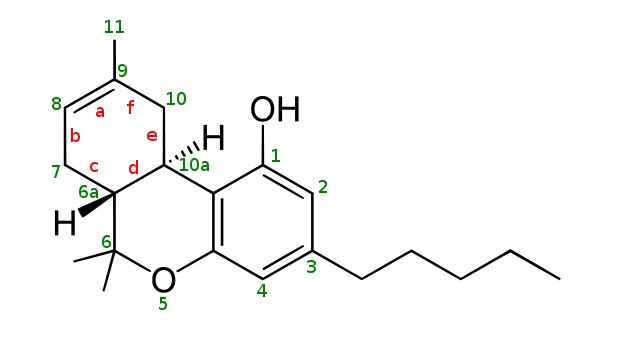
\includegraphics[width=0.4\textwidth]{Images/Trucs/Delta-8-THC.jpg}
			\label{sub:delta8}
		}
		\subfloat[Isomère \Deltatext{9}]{
			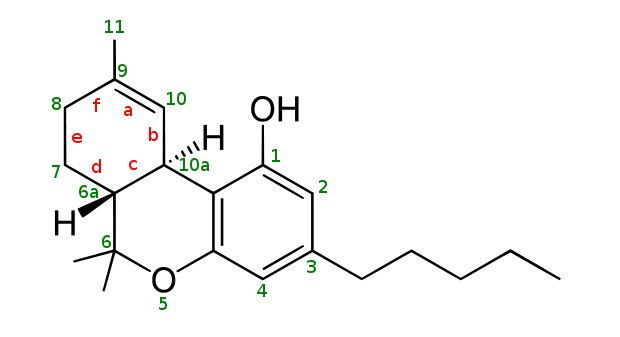
\includegraphics[width=0.4\textwidth]{Images/Trucs/Delta-9-THC.jpg}
			\label{sub:delta9}
		}
		\caption{Deux isomères du \THC}
		\label{fig:isomereTHC}
	\end{center}
\end{figure}
\end{frame}

\begin{frame}
\frametitle{L'heure du TP !}
Notons que le \THC \hspace{0.1cm}(de formule \formule{21}{30}{2} je le rappelle) possède des vertus anti-inflammatoires et anti-métastatiques\footnote{Bonjour\url{https://fr.wikipedia.org/wiki/T\%C3\%A9trahydrocannabinol}}.\\
.\\
.\\
.\\

[1] \href{https://fr.wikipedia.org/wiki/T\%C3\%A9trahydrocannabinol}{Wikipedia} le dit (mot cliquable, note de bas de page ou référence).

\end{frame}

\begin{frame}[fragile=singleslide]
	\frametitle{Solution}
\begin{verbatim}
% Préambule

\usepackage{subscript}
\newcommand{\THC}{tétrahydrocannabinol}
\newcommand{\formule}[3]{\textbf{C}\textsubscript{#1}
\textbf{H}\textsubscript{#2}\textbf{O}\textsubscript{#3}}
\newcommand{\Deltatext}[1]{$\Delta$\up{#1}}
\end{verbatim}
	
\end{frame}

\begin{frame}[fragile=singleslide]
\frametitle{Solution}
\begin{verbatim}
% 1ère slide

\begin{block}{Notations}
On note \textit{THC} le \THC. Il possède comme formule 
brute \formule{21}{30}{2}.
\end{block}
\end{verbatim}

\end{frame}


\begin{frame}[fragile=singleslide]
\frametitle{Solution}
\footnotesize
\begin{verbatim}
% 1ère slide
Ce cannabinoïde possède plusieurs isomères :\\
\begin{figure}[h]
	\begin{center}
		\subfloat[Isomère \Deltatext{8}]{
			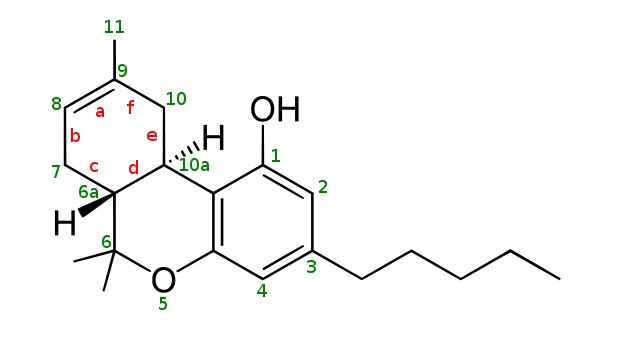
\includegraphics[width=0.4\textwidth]{Images/Trucs/Delta-8-THC.jpg}
			\label{sub:delta8}
		}
		\subfloat[Isomère \Deltatext{9}]{
			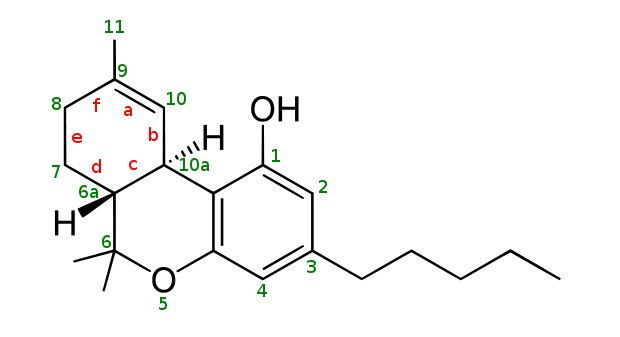
\includegraphics[width=0.4\textwidth]{Images/Trucs/Delta-9-THC.jpg}
			\label{sub:delta9}
		}
		\caption{Deux isomères du \THC}
		\label{fig:isomereTHC}
	\end{center}
\end{figure}
\end{verbatim}
\end{frame}

\begin{frame}[fragile=singleslide]
\frametitle{Solution}
\footnotesize
\begin{verbatim}
% 2ème slide

Notons que le \THC \hspace{0.1cm}(de formule \formule{21}{30}{2} 
je le rappelle) possède des vertus anti-inflammatoires et 
anti-métastatiques 
\footnote{
\href{https://fr.wikipedia.org/wiki/T\%C3\%A9trahydrocannabinol}
{Wikipedia} 
le dit.}.

\end{verbatim}
\end{frame}

\begin{frame}
	\frametitle{Do not forget}
	\centering
	\begin{quote}
		RTFM.
	\end{quote}
\end{frame}

\section{Les classes, les extensions, les thèmes, les trucs qui simplifient la vie}

\begin{frame}
\frametitle{Embellissons...}
Dans ce qu'on a vu jusqu'à présent :
\begin{enumerate}
	\item Le thème \textit{Warsaw} n'est pas incroyable, et les autres disponibles par défaut ne sont pas non plus glorieux...
\end{enumerate}
\end{frame}

\begin{frame}
\frametitle{Embellissons... et simplifions}
Dans ce qu'on a vu jusqu'à présent :
\begin{enumerate}
	\item Le thème \textit{Warsaw} n'est pas incroyable, et les autres disponibles par défaut ne sont pas non plus glorieux...
	\item On utilise des packages à foison au début de chaque document \LaTeX \vspace{1cm} et obligé de faire C/C à chaque fois
\end{enumerate}
\end{frame}

\begin{frame}
\frametitle{Comment avons-nous un template KI ?}
	D'où l'utilité des fichiers \textit{.sty} (fichiers d'extensions). Pour faire cette présentation, on a besoin de :
	\begin{itemize}
		\item \textit{beamercolorthemeki.sty} // Couleurs
		\item \textit{beamerinnerthemeki.sty} // A l'intérieur de chaque frame
		\item \textit{beamerouterthemeki.sty} // Bandeau d'une frame
		\item \textit{beamerthemeki.sty} // Combine le tout
	\end{itemize}
\end{frame}

\begin{frame}[fragile=singleslide]
\frametitle{Comment avons-nous un template KI ?}
Dans le \textit{beamertheme.sty} :
\begin{verbatim}
\mode<presentation>
% Requirement
\RequirePackage{tikz}

\definecolor{ki}{RGB}{44, 45, 45}

% Settings
\useinnertheme{ki}
\useoutertheme{ki}
\usecolortheme{ki}

\setbeamertemplate{navigation symbols}{}
\mode<all>
\end{verbatim}
\end{frame}

\begin{frame}[fragile=singleslide]
\frametitle{Comment avons-nous un template KI?}
Dans le \textit{beamercolortheme.sty} :
\begin{verbatim}
\mode<presentation>

% Settings
\setbeamercolor*{title}{fg=white}
\setbeamercolor*{title page header}{fg=white}
\setbeamercolor*{author}{fg=white}
\setbeamercolor*{date}{fg=white}
\setbeamercolor*{item}{fg=orange}
\setbeamercolor*{background canvas}{bg=ki}
\setbeamercolor*{footline}{fg=ki}
\setbeamerfont*{footline}{series=\bfseries}

\mode<all>
\end{verbatim}
\end{frame}

\begin{frame}
\frametitle{Simplifions l'importation des packages !}
Certains packages sont toujours à importer : \\ \textit{babel}, \textit{inputenc}, \textit{fontenc}\\
D'autres sont souvent nécessaires : \\
\textit{graphicx}, \textit{float}, \textit{amssymb}, \textit{amsmath}, etc.
\end{frame}

\begin{frame}
\frametitle{Simplifions l'importation des packages !}
Certains packages sont toujours à importer : \\ \textit{babel}, \textit{inputenc}, \textit{fontenc}\\
D'autres sont souvent nécessaires : \\
\textit{graphicx}, \textit{float}, \textit{amssymb}, \textit{amsmath}, etc.\\

\hspace{5em}
\fbox{
La meilleure solution pour regrouper tout ça : 
\textit{monextension.sty}
}
\end{frame}

\begin{frame}[fragile=singleslide]
\frametitle{Simplifions l'importation des packages !}
A l'intérieur :\\
\begin{verbatim}
\NeedsTeXFormat{LaTeX2e} 
% Format pour lequel cette extension est créée,
% LaTeX2e est la version stabilisée la plus récente 
% de LaTeX (le langage informatique)

\ProvidesPackage{monextension}[26/02/2019, 
Ma Meilleure Extension, Version 12.04] 
% Petite description, nom du fichier sans le .sty
\end{verbatim}
\end{frame}

\begin{frame}[fragile=singleslide]
\frametitle{Simplifions l'importation des packages !}
\begin{verbatim}
% extensions

\RequirePackage[latin1]{inputenc}
\RequirePackage[T1]{fontenc}
\RequirePackage{lmodern}
\RequirePackage{graphicx}
\RequirePackage[frenchb]{babel}

% commandes personnelles

\newcommand{\bff}{koukou}
\newcommand{\michesdepain}{Andréas & Nicolas}
\end{verbatim}
\end{frame}

\begin{frame}[fragile=singleslide]
\frametitle{Simplifions l'importation des packages !}
\framesubtitle{Et dans le \textit{.tex} ?}
\begin{verbatim}
\documentclass[a4paper, 11pt]{article}

% Comme un package normal en somme, 
% mais il n'y en a plus beaucoup !
\usepackage{monextension} 

\begin{document}
...
\end{verbatim}


\centering 
Pratique pour factoriser l'utilisation de ses packages !

\end{frame}


\begin{frame}
	\centering
	\Huge
	\textsc{MERCI BEAUCOUP !}\\
	\vspace*{2cm}
	\normalsize
	\textsc{Le KI '020}\\
	\vspace*{1cm}
	\centering
	
\includegraphics[scale=0.2]{logo-ki.png}
\end{frame}



\end{document}
